\documentclass[../main.tex]{subfiles}

\begin{document}

\chapter{Multi-armed bandits}\label{bandit}

At the beginning of the thesis \refsec{bg:mdp}, we discussed the Markov decision process as one of the models used for describing a single-agent environment.
In MDPs, an agent continuously chooses actions by which he moves through many states of the environment and receives rewards throughout the process.
Moreover, this model can be used for learning agent's optimal actions and policies in each state.

This section is about examining MDPs where the set of all states $S$ is a singleton, i.e. consists of only one state $s \in S$.
This subset of all MDPs is often referred to as \textit{Multi-armed bandits} and many algorithms based on this model are very useful for solving more complex problems.
The bandits are a well-known tool of reinforcement learning enabling a single agent to gain information about the environment and leverage it for its advantage.
Here, we describe the basic concepts of bandit learning and provide multiple specific algorithms designed for this purpose.

This section and the standard versions of the bandit algorithms are based on a book \textit{Introduction to Multi-Armed Bandits}\cite{bandits}.

\section{Basics}\label{bandit:basics}
As stated above, a Multi-armed bandit problem is essentially a Markov decision process of a single state $s \in S$ with many, possibly infinitely many, different available actions $a_i \in A$.
In the context of bandit algorithms, these actions are called 'arms' and hence the adjective \textit{multi-armed}.
We will use 'arms' and 'actions' interchangeably within this chapter.
\begin{figure}[ht]
    \centering
    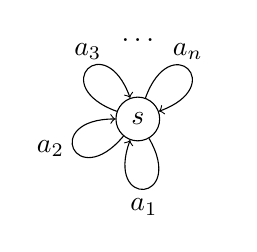
\begin{tikzpicture}[state/.style={draw, circle}]
        \node[state] (0) {$s$};
        \node[above of=0] (1) {$\dots$};
        \draw[->] (0) to [out=70, in=20, looseness=10] node[midway, above] {$a_n$} (0);
        \draw[->] (0) to [out=160, in=110, looseness=10] node[midway, above] {$a_3$} (0);
        \draw[->] (0) to [out=230, in=180, looseness=10] node[midway, left] {$a_2$} (0);
        \draw[->] (0) to [out=300, in=250, looseness=10] node[midway, below] {$a_1$} (0);
    \end{tikzpicture}
    \caption{Model of a multi-armed bandit}
    \label{bandit:basics:model}
\end{figure}
There exists a variety of different bandit algorithms, which can be used in many contexts.
By using them, one can decompose a complex problem into many smaller bandit problems, which can learn independently on the others.
The means and methods of bandit learning are presented in the next part.

\section{Bandit learning}\label{bandit:learn}
Let's suppose that the rewards of actions depend solely on the current state.
In other words, the rewards are identically independently distributed.
Thus, a bandit learning a particular state can learn independently on the other bandits.

The bandit learning takes place in discrete time steps $t = 1, \dots$.
In each step $t$, the bandit selects and plays an arm $a^t \in A$ according to some decision rule and receives a reward $r^t$.
This decision rule, or sometimes selection rule, is the main distinction point among the many multi-armed bandit algorithms.
The bandit stores the received rewards, updates its inner state and uses them for the next arm selections.

As a basis for the arm selection process, it is convenient to have some measure of quality of a function.
For this purpose, we define so-called action function $q^*: A \to \mathbb{R}$
\begin{equation}\label{bandit:learn:opt}
    q^*(a) = \mathbb{E}[r^t \mid a^t = a] \quad \forall a \in A.
\end{equation}

However, neither the optimal values $q^*(a)$, nor the distribution the rewards are drawn from, is not known by the algorithm.
Thus, instead of the true values for actions, it estimates these values by averaging received rewards over time.
For this purpose we define an action function estimate $Q^t: A \to \mathbb{R}$ in time step $t$, corresponding to the average reward gained by playing some action $a \in A$ so far.
\begin{definition}\label{bandit:learn:afunc}
    Let $A$ be a set of all arms of a bandit algorithm and $t \in \mathbb{N}$ be the current time step. Then, $Q: A \to \mathbb{R}$ is defined as
    \begin{equation}
        Q^t(a) = \frac{\sum_{i = 1}^{t}r^i\cdot\llbracket a^i = a \rrbracket}{\sum_{i = 1}^{t}\llbracket a^i = a \rrbracket} \quad \forall a \in A, 
    \end{equation}
    the indication function $\llbracket.\rrbracket$ is defined as
    \begin{equation}
        \llbracket a^i = a \rrbracket = \begin{cases}
            1 & a^i = a \\
            0 & a^i \neq a
        \end{cases}
    \end{equation}
    and where $a^i$ is an action taken in time step $i \in {1, \dots, t}$ and $r^i$ is reward gained by playing this action $a^i$.
\end{definition}

Even though this formula is clear and simple it is not very computationally efficient, because it would require evaluating two sums every time.

First, we need to derive an incremental computation of an arithmetic average of values.
Let $X_{m}$ be an arithmetic average of first $m - 1$ values $x_1, \dots, x_{m - 1}$, where
\begin{equation}\label{bandit:learn:incrementalavg}
    X_{m} = \frac{x_1 + x_2 + \cdots + x_{m - 1}}{m - 1}.
\end{equation}
Then, the arithmetic average of values received before time step $m + 1$ can be computed as
\begin{equation}\label{bandit:learn:incrementalavg:derivation}
    \begin{split}
        X_{m+1} &= \frac{1}{m}\sum_{i = 1}^{m}x_i = \frac{1}{m}\sum_{i = 1}^{m - 1}x_i + \frac{1}{m}x_m = \frac{m - 1}{m - 1}\frac{1}{m}\sum_{i = 1}^{m - 1}x_i + \frac{1}{m}x_m =\\
        & = \frac{m - 1}{m}\frac{1}{m - 1}\sum_{i = 1}^{m - 1}x_i + \frac{1}{m}x_m = \frac{m - 1}{m}X_m + \frac{1}{m}x_m = \\
        & = \frac{m}{m}X_m - \frac{1}{m}X_m + \frac{1}{m}x_m = X_m + \frac{x_m - X_m}{m}
    \end{split}
\end{equation}
Now, we can describe the computation of the action function estimate $Q^t$.
Instead of keeping a full action-reward history, a bandit algorithm keeps track of the current average of received values so far in $Q^t(a) ,\, \forall a \in A$ and also how many times have been each action selected in a vector $n(a) \in \mathbb{N}^{\left|A\right|}$.
On receiving reward $r^t$ after playing action $a^t$, the trial function is trivially updated as
\begin{equation}
    n^{t+1}(a^t) = n^{t}(a^t) + 1.
\end{equation}
The update $Q^{t+1}(a^t)$ can be computed by employing the previously derived incremental averaging rule for the action selected at this time round.
\begin{equation}\label{bandit:learn:Qupdate}
    Q^{t+1}(a) = \begin{cases}Q^t(a) + \frac{r^t - Q^t(a)}{n^{t+1}(a)} & a^i = a \\ Q^t(a) & \text{otherwise}\end{cases} \quad \forall a \in A
\end{equation}
Notice that except the changed notation, the update is the same as the result of \refeq{bandit:learn:incrementalavg}.

\subsection{Exploration-exploitation trade-off}\label{bandit:learn:expexp}
Action $a^t$ for which it holds
\begin{equation}\label{bandit:learn:expexp:greedyaction}
    a^{t} \in \argmax_{a \in A} Q^t(a),
\end{equation}
is usually called the \textit{greedy action}.
In some sense, it is the best of all possible actions with respect to the received rewards up to the time step $t$.

However, always selecting the greedy action, which could be then called a \textit{greedy bandit}, can cause problems or slow down the convergence of the function $Q^t$ to the optimal action function $q^*$ and thus making it harder for the bandit algorithm to find the optimal actions to play.
To improve convergence to the real values and prevent getting stuck in some local optima, the \textit{exploration-exploitation trade-off} has to be taken into account.

\textit{Exploration} is a mechanism when a multi-armed bandit explores possibilities, i.e. actions, that either have not yet been selected or the so far collected average reward is much lower than for other actions and thus are not selected by the greedy method.
\textit{Exploitation}, on the other hand, is abusing so far learned values to take as much profit as possible.
In other words, exploitation is selecting the action, which is thought to provide the highest reward.
It is essential for a well-performing bandit algorithm to balance these two aspects in some way.
If it was too much exploration, by selecting actions with values very different from the real value, it would take a long time to converge and find the optimum.
If it was too much exploitation, it would get likely stuck in some local optima and it would struggle to find the best actions to select.

Now we have everything ready to present some common bandit algorithms with several arm selection rules, which handle the exploration-exploitation trade-off differently.

\section{Stochastic bandits}\label{bandit:stochastic}
Stochastic bandits are the simplest multi-armed bandit algorithms mentioned in this thesis.
As mentioned before, the rewards are assumed independent and identically distributed as well as bounded.

At first, the $Q$ function and function counting action trials $n$ are initialized.
\begin{algorithm}
    \caption{\textbf{Initialize} a bandit}
    \label{bandit:stochastic:init}
    \begin{algorithmic}[1]
        \Require action set $A$
        \State $Q(a) \leftarrow 0 \quad \forall a \in A$
        \State $n(a) \leftarrow 0 \quad \forall a \in A$
    \end{algorithmic}
\end{algorithm}

In each time step $t$ the algorithm selects an arm $a^t$.
After, the standard versions of these bandit algorithms observe only the received reward $r^t$, which is then called \textit{bandit feedback}.
\begin{algorithm}[ht]
    \caption{The \textbf{receive} function for \textit{bandit feedback}}
    \label{bandit:stochastic:receive}
    \begin{algorithmic}[1]
        \Require $n$, $Q$, action $a^t$, reward $r^t$
        \State $n(a^t) \leftarrow n(a^t) + 1$
        \State $Q(a^t) \leftarrow Q(a^t) + \frac{r^t - Q(a^t)}{n(a^t)}$
    \end{algorithmic}
\end{algorithm}
However, in the context of games, we later construct \textit{observable} variants \refsec{new:bandit:obs} for each mentioned stochastic bandit algorithm, which also observes the action taken by the opponent $a^{\prime}_{t}$.
Later in this thesis, we will compare the observable and standard alternatives and see if the information about the opponent's selections can be leveraged and will lead to faster convergence.

Now, we define the standard stochastic bandit algorithms.
The first two mentioned bandits are often termed as \textit{non-adaptive} because they do not adjust the amount of exploration during the course of learning.

\subsection{Best of $N$}\label{bandit:stochastic:bestofn}
\begin{algorithm}
    \caption{\textbf{Best of $N$} bandit}
    \label{bandit:stochastic:bestofn:alg}
    \begin{algorithmic}[1]
        \Require action set $A$, $N \in \mathbb{N}$
        \State try arms uniformly at random until each one was tried exactly $N$ times
        \State select the action greedily as $a_{\text{greedy}} \leftarrow \argmax_{a \in A} Q(a)$
        \State play $a_{\text{greedy}}$ forever
    \end{algorithmic}
\end{algorithm}
The first and simplest bandit algorithm described in this thesis is a \textit{Best of $N$} bandit \refalg{bandit:stochastic:bestofn:alg}, sometimes known as an \textit{uniform} bandit.
It has a single parameter $N \in \mathbb{N}$ which influences the degree of exploration of each action.
In short, the bandit uniformly tries actions and accumulates the average received rewards until each action was tried exactly $N$ times.
After all actions has been tried $N$ times, exploration ends and from that point, the algorithm only exploits.
The exploitation phase is very simple as the agent selects the greedy action $a_{\text{greedy}}$ \refdef{bandit:learn:expexp:greedyaction} and plays it forever.

\subsection{$\epsilon$-greedy}\label{bandit:stochastic:epsgreedy}
\begin{algorithm}
    \caption{\textbf{$\epsilon$-greedy} bandit}
    \label{bandit:stochastic:epsgreedy:alg}
    \begin{algorithmic}[1]
        \Require action set $A$, $\epsilon \in \left[0, 1\right]$
        \State with probability $\epsilon$ sample $a^t$ uniformly from $A$
        \State with probability $\left(1 - \epsilon\right)$ select the greedy action $a^t \leftarrow \argmax_{a \in A} Q(a)$
    \end{algorithmic}
\end{algorithm}
The second bandit algorithm, which we will discuss here is an \textit{$\epsilon$-greedy} bandit \refalg{bandit:stochastic:epsgreedy:alg}.
In contrast to the Best of N bandit, $\epsilon$-greedy does not separate exploration and exploitation phases so strictly but does it in a more clever way founded on a single parameter $\epsilon \in [0, 1]$.
At the beginning of every action selection process, the algorithm probabilistically chooses between two possibilities.
With probability $\epsilon$, it chooses exploration and samples action $a^t$ from uniform distribution over the set $A$.
Otherwise, with probability $\left(1 - \epsilon\right)$, it selects greedy action based on saved function $Q^t$ as in \refdef{bandit:learn:expexp:greedyaction}.

The parameter $\epsilon$ thus controls how often the algorithm explores and how often it exploits.
A typical value of $\epsilon$ is $0.1$, which means that exploration is expected to occur every $10^{\textit{th}}$ round.
However, this value can be tuned to a specific problem.
If $\epsilon = 0$, then the bandit degrades to a \textit{greedy} bandit, which never explores and only chooses the action with highest accumulated rewards $Q^t$.

As opposed to Best of $N$ and $\epsilon$-greedy stochastic bandits, both non-adaptive multi-armed bandits, the following two algorithms are \textit{adaptive}, because exploration of an arm depends on a \textit{confidence} that the accumulated average rewards are a good approximation of the real values.
For the purpose of this and the next bandit, we need to define \textit{confidence interval} and \textit{confidence bounds}.

A confidence interval is a range around the estimated value and it holds that the true value lies in this range with high probability.
The two limit points of this said interval are \textit{confidence bounds}, \textit{lower} and \textit{upper}.
We will use such confidence bounds as were derived in \cite{bandits} using \textit{Hoeffding Inequality}.
\begin{definition}\label{bandit:stochastic:confidence}
    For each arm $a$ at fixed time step $t$ let $n^t(a)$ represent the number of selections of the arm $a$ before time $t$ and $Q^t(a)$ is the accumulated mean reward until $t$.
    We then define a \textit{confidence radius} $r^t(a)$ as derived in \cite{bandits}:
    \begin{equation}
        r^t(a) = \sqrt{\frac{2 \log{t}}{n^t(a)}}.
    \end{equation}
    Let $\alpha \in \mathbb{R}, \alpha \geq 0$ be a parameter.
    The upper confidence bound, resp. lower confidence bound is thus defined as
    \begin{equation}
        \ucbt = Q^t(a) + \alpha \cdot r^t(a)
    \end{equation}
    \begin{equation}
        \lcbt = Q^t(a) - \alpha \cdot r^t(a)\\
    \end{equation}
    Hence, the confidence interval of an estimate $Q^t(a)$ is $[\lcbt, \ucbt]$.
\end{definition}
Now we have everything ready to present the two \textit{adaptive} stochastic bandit algorithms.

\subsection{Successive elimination}\label{bandit:stochastic:succelim}
\begin{algorithm}
    \caption{\textbf{Successive elimination} bandit}
    \label{bandit:stochastic:succelim:alg}
    \begin{algorithmic}[1]
        \Require action set $A$, $\alpha \in \mathbb{R}_{+}$
        \State set all actions as \textit{active} arms
        \Statex
        \State try each \textit{active} arm once
        \State deactivate every active arm $a$ for which $\ucbt \leq \lcbtp$ for some other active arm $a^{\prime}$
    \end{algorithmic}
\end{algorithm}
\textit{Successive elimination} bandit \refalg{bandit:stochastic:succelim:alg} tries all actions until it is confident, based on the computed confident intervals, that some action is the best.
From that point, it plays only this best action forever.
The bandit keeps a set of \textit{active} arms, which is initialized to contain all possible actions.
It iteratively selects actions from this active set one by one until it tries every arm.
After each active arm was tried, it computes the confidence bounds $\lcb$ and $\ucb$ for each arm $a$ in current time step $t$.
Then, if for some active arm $a$ and some other active arm $a^{\prime}$ holds
\begin{equation}\label{bandit:stochastic:succelim:deactivation}
    \ucbt \leq \lcbtp
\end{equation}
the action $a$ is \textit{deactivated}, i.e. removed from the active set.
The condition \refineq{bandit:stochastic:succelim:deactivation} is often called the \textit{deactivation rule}.
After this rule is applied to each previously active arm, the algorithm starts again iteratively selecting arms from this newly constructed active set.
This continues until only a single action remains.
Then, the intervals need not be computed and only the remaining action is selected until the end.

The deactivation rule can be visualized on the confidence intervals.
When the intervals of two different actions overlap, it cannot be said, that one is better than the other, with enough confidence.
However, if the intervals are disjoint, the arm with a lower average reward simply cannot be better with high enough probability and thus can be deactivated.

The exploration parameter $\alpha$ in the computation of upper confidence bound values, resp. lower confidence bound values, influences how much one trial improves the confidence of the estimate.
Higher values mean more trials are needed to gain enough confidence about the average of received values.

\subsection{UCB}\label{bandit:stochastic:ucb}
\begin{algorithm}
    \caption{\textbf{UCB} bandit}
    \label{bandit:stochastic:ucb:alg}
    \begin{algorithmic}[1]
        \Require action set $A$, $\alpha \in \mathbb{R}_{+}$
        \State always select $a^t \in \argmax_{a \in A} \ucb$
    \end{algorithmic}
\end{algorithm}
The idea behind \textit{UCB} bandit, or fully \textit{Upper Confidence Bound} bandit, is simpler than behind Successive elimination as it does not consider lower confidence bound at all, but it often performs better and is more widely used than Successive elimination.
It does not deactivate arms, but every time step $t$ it directly selects the action $a$ with the highest $\ucb$ value.
In other words, UCB bandit selects the action, which is optimistically the best, or that has the best potential outcome based on the rewards received so far.
As in successive elimination bandit, it has a single parameter $\alpha \in \mathbb{R}, \alpha \geq 0$, which controls the amount of exploration, specifically, how fast the confidence bounds get tighter with one trial.

\section{Adversarial bandits}\label{bandit:adversarial}
So far, all stochastic bandits were using so-called \textit{bandit feedback}.
In other words, they received only the reward gained by playing the selected action, but the potential rewards for other actions remained unknown.
\textit{Adversarial} bandits not only receive the reward for the chosen action, they also observe all the other rewards.
This is called \textit{full feedback}.
However, the applications of bandits do not always enable receiving rewards for all actions, so later, a way to use bandit feedback to fit into the full feedback model will be shown.

Moreover, adversarial bandits do not assume i.i.d. rewards, instead they are arbitrarily chosen by an unknown virtual adversary, thus the name adversarial.
For example, while UCB is designed to learn the best pure strategy, i.e. always play the single best action, the adversarial bandits strive to find suitable probability distributions over possible actions and thus learn mixed strategies.
This phenomenon is discussed on examples in a later chapter.

\subsection{Hedge algorithm}\label{bandit:adversarial:hedge}
The main idea from this category of bandits, which is used in further introduced bandits, is expert advice.
An expert can be viewed simply as a function, which gives its prediction, or advice, about the action to play.
The algorithm has a set of experts $E$ and in each time step decides which expert's advice to follow.
For this purpose serves the \textit{Hedge} algorithm.

The purpose of this algorithm is to evaluate performance of individual experts in a sense whether their advice was fulfilled or not and based on this adjust how often the particular expert is followed.
To ensure some amount of exploration, the expert selection is done in a way of assigning weights to the experts and sampling the current expert from a distribution proportional to these assigned weights.
In this setting, it is not a full bandit algorithm, it is more of a core algorithm for some other adversarial bandit which enwraps it and uses its weighting system to handle the experts.

\begin{algorithm}
    \caption{\textbf{Hedge} algorithm}
    \label{bandit:adversarial:hedge:alg}
    \begin{algorithmic}[1]
        \Require the set of experts $E$, parameter $\epsilon \in \left(0, \frac{1}{2}\right)$
        \State Initialize weights $w^1(e) \leftarrow 1 \quad \forall e \in E$
        \For {$t \leftarrow 1, \dots$}
            \State construct probability distribution $p^t(e) = \frac{w^t(e)}{\sum_{e^{\prime} \in E} w^t(e^{\prime})} \quad \forall e \in E$
            \State sample expert: $e \sim p^t\left(.\right)$
            \State observe rewards: $r^t(e) \quad \forall e \in E$
            \State adjust weights: $w^{t+1}(e) \leftarrow w^t(e) \cdot (1 - \epsilon)^{-r^t(e)} \quad \forall e \in E$
        \EndFor
    \end{algorithmic}
\end{algorithm}

Input to this algorithm is the set of experts $E$ and a single parameter $\epsilon \in \left(0, \frac{1}{2}\right)$, which determines how much do received rewards change the weights.
The initial weight of every expert is set to $w^1(e) = 1$, $\forall e \in E$, so at the beginning, all bandits have the same probability of selection.

In each time step $t$ a probability distribution $p$ over the set of experts $E$ is constructed as
\begin{equation}\label{bandit:adversarial:hedge:prob}
    p^t(e) = \frac{w^t(e)}{\displaystyle\sum_{e^{\prime} \in E} w^t(e^{\prime})} \quad \forall e \in E
\end{equation}
From this distribution $p^t$ the algorithm samples an expert, whose advice will be used in this time step $t$.
Based on the observed rewards for every expert $r^t(e)$, new weights are computed based on the arm they recommended.
\begin{equation}\label{bandit:adversarial:hedge:weight}
    w^{t+1}(e) = w^t \cdot (1 - \epsilon)^{-r^t(e)} \quad \forall e \in E
\end{equation}
In the cited textbook \cite{bandits}, this algorithm is defined for costs rather than for rewards, hence the extra minus sign before $r^t(e)$ in the exponent of weight update.

Now we present a bandit algorithm using Hedge to achieve balance between exploration and exploitation and provide good arm selection, while requiring bandit feedback, which is natural to many bandit use cases.

\subsection{Exp3}\label{bandit:adversarial:exp3}
First, we need to discuss how to adapt bandit feedback, so that is accepted by the Hedge algorithm, which requires full feedback.
It is necessary because bandit feedback is more common in bandit algorithms as the environment rarely returns rewards for all possible actions, but only the actual outcome.
This obstacle can be tackled by using \textit{fake costs}.

\begin{algorithm}
    \caption{\textbf{Exp3} bandit}
    \label{bandit:adversarial:exp3:alg}
    \begin{algorithmic}[1]
        \Require action set $A$, $\epsilon \in \left(0, \frac{1}{2}\right)$, $\gamma \in \left[0, \frac{1}{2}\right)$
        \State create set of experts $E \leftarrow \left\{e: e_a = a^{\prime} \mid \forall a^{\prime} \in A\right\}$
        \For {$t \leftarrow 1, \dots$}
            \State retrieve expert probabilities $p^t$ from hedge
            \State sample an expert $e^t \sim \{p^t\}$
            \State with probability $(1 - \gamma)$ use action $a^t = e^t_a$ recommended by sampled expert $e^t$, otherwise sample action $a^t$ uniformly at random
            \State observe immediate reward $r^t(a^t)$
            \State compute fake costs $\hat{r}^t(.)$ according to \refform{bandit:adversarial:exp3:fakecosts}
            \State return fake costs $\hat{r}^t(.)$ to hedge
        \EndFor
    \end{algorithmic}
\end{algorithm}

As said before, the \textit{Exp3} adversarial bandit is built on top of the Hedge algorithm \refalg{bandit:adversarial:hedge:alg} and provides a transition from bandit feedback to fake costs.
Experts in Exp3 are constructed trivially as for one possible action $a_i \in A$ exists exactly one expert $e_i \in E$, which always recommends said action $a_i$.
No other experts are present in the set of all experts, except those mentioned above.
In addition to the Hedge parameter $\epsilon \in \left(0, \frac{1}{2}\right)$, Exp3 takes a parameter $\gamma \in \left[0, \frac{1}{2}\right)$, which regulates additional exploration.

In each time step $t$, the algorithm receives probability $p^t$ over experts from Hedge.
Exploration is provided by a procedure similar to $\epsilon$-greedy bandit.
With probability $\gamma$ the algorithm samples a random action uniformly from the set of all possible actions.
Otherwise, it samples an expert $e^t$ from the Hedge probability $p^t$ and follows its advice $e^t_a$.
Let the selected action be denoted $a^t$ independent of how it was selected.
From the received reward for the chosen (sampled or recommended) action the fake rewards $\hat{r}^t$ are computed by a formula
\begin{equation}\label{bandit:adversarial:exp3:fakecosts}
    \hat{r}^t(e) = \begin{cases} \frac{r^t(a)}{\text{Pr}\left[a^t = e^t_a \mid p^t\right]} & a^t = e^t_a, \\ 0 & \text{otherwise}\end{cases}.
\end{equation}
These rewards are then returned to Hedge as real rewards to update its inner expert weights.

This time, exploration is regulated by two parameters.
$\gamma$ influences the more aggressive exploration with random actions, while $\epsilon$ manages selection of experts, which do not predict so well very often.

There exists an extension of the Exp3 algorithm, which is called Exp4 and differs in used experts.
The user can define arbitrary experts to predict future actions and the number of experts does not even need to coincide with the number of possible actions.
However, this bandit algorithm was not used in this thesis.

\section{Summary}
In this chapter, we focused on learning in an environment using multi-armed bandit algorithms.
The most simple stochastic bandits were described in addition to the more complex adversarial bandit algorithm Exp3 \refsec{bandit:adversarial:exp3}.
Although, these methods are designed for a single agent, they can be used to play games as well.
In the next section, we propose modifications to make them fit more into algorithms solving games, stochastic games specifically.

\end{document}

